\section{Introduction}
Human innovation is not only a generative capacity for creativity, but also includes the ability to evaluate the subjective quality of new ideas and artifacts. Great ideas are rarely generated all at once out of whole cloth, but rather gradually emerge through divergent chains of elaboration and revision \citep{stanley2015greatness}. To successfully navigate such a tree of ideas, the creator must evaluate which steps in a chain are worth pursuing further, a question that can be highly subjective, especially in domains with artistic or literary dimensions.

Until now, even if AI could provide candidates, the hope for such subjectively tinged evaluation lay firmly with humans. However, the emerging foundation model technology of recent years \citep{bommasani2021opportunities} now means that the model can also play the role of evaluator, even when the evaluation is in part subjective \citep{madaan2023self}. In this way, for the first time, an entire ideation process that returns a diverse set of interesting artifacts can in principle be automated. This process cannot be run by LMs entirely on their own, but requires chaining together a search algorithm with model calls in a nuanced way. This paper highlights one way to achieve this potential: to combine LMs with the field of quality-diversity (QD) \citep{mouret2015illuminating}, which centers on how to design search processes that produce high-quality solutions that span a design space.

The main insight in QD algorithms is to explicitly maintain and seek high-quality diverse responses. Typically such search algorithms require hand-designed measures of diversity and quality, as well as a way to generate meaningful variation. Yet the most interesting and complex domains nearly always involve notions of performance, diversity, and variation that are subjective or difficult to specify algorithmically. Extending work that generates variation through LMs \citep{lehman2022evolution, meyerson2023language} and evaluates the quality of potential solutions through LMs \citep{ahn2022can}, we show that LMs can also be used to evaluate qualitative aspects of diversity. In this way, LMs can instantiate the three main ingredients of QD search, thereby enabling powerful new QD algorithms that can ride the coattails of continual LM advances, which we name Quality-Diversity through AI Feedback (QDAIF). Such QDAIF can explore and return diverse, high-quality responses to an LM prompt through more-intuitive diversity measures, without the need for model fine-tuning (although, it could also be used for LMs to self-improve by generating fine-tuning data \citep{lehman2022evolution, chen2023evoprompting}), an interesting direction for self-curated effective learning environments via generated data, towards AI-generating algorithms \citep{clune2019ai}).

We evaluate QDAIF across three creative writing domains: opinion writing, short stories, and poetry. The idea is that in such creative domains, users often enjoy seeing a wide range of possible stories or poems from which to choose or be inspired by. Quantitative results indicate that QDAIF significantly outperforms existing baselines. Additionally, through human evaluation, we observe a strong alignment between human and AI-generated feedback, providing empirical evidence that AI feedback is grounded and that the method can work in practice (i.e.\ it yields improved quality and diversity as measured by humans). Overall, QDAIF brings us a step closer to AI models that can independently search and innovate, one of the keystone abilities of humans that allow them to create culture and science \citep{stanley2017open}.

\begin{figure}[t]
    \centering
    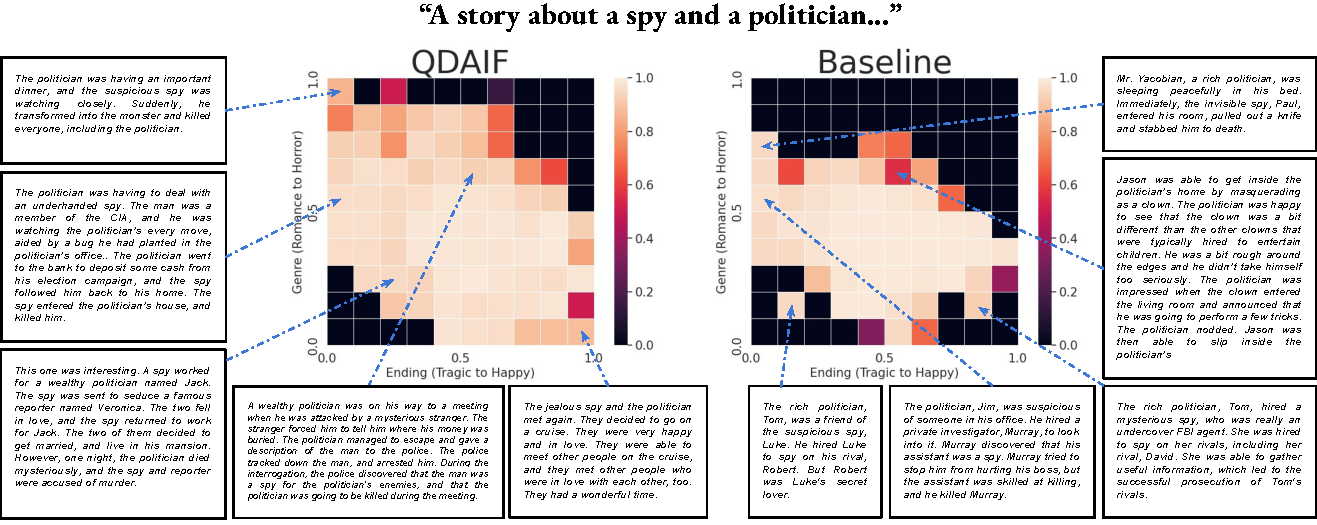
\includegraphics[width=\textwidth]{main_figures/Heatmap_Figure.pdf}
    \vspace{-0.7cm}
    \caption{\textbf{QDAIF (left) covers more the search space with diverse, high-quality stories compared to the baseline (right).} The baseline is \basefour{} \citep{meyerson2023language}, which optimizes only for the quality of solutions. QDAIF discovered more interesting stories about a spy and a politician, covering examples such as romance stories with a happy-ending, to horror stories with a tragic-ending. The baseline produced a story (right-middle position, starting with "Jason") with a lower quality score due to the lack of a desired spy character (denoted by the red-colored bin, for a story with a neutral ending, and leaning to horror). QDAIF discovered a better, more-relevant story (bottom-middle position, starting with "a wealthy politician") for this same neutral bin.}
    \label{fig:overview}
\end{figure}

